%------------------------------------------------------------------------------
\section{Konfiguration des DNS-Servers mit BIND}
%------------------------------------------------------------------------------
Im Folgenden wird nun der Server \textbf{srv200} als Nameserver konfiguriert.
Hier wird wieder exemplarisch die Konfiguration von \textbf{srv200} wiedergegeben.
Die für Sie benötigten Werte entnehmen Sie bitte aus der Tabelle im Anhang.
Melden Sie sich wieder am Server \textbf{srv200} mit den bekannten Zugangsdaten
an. Danach wird nun die Software \textbf{bind} installiert.

\begin{lstlisting}
admin1@srv200$ sudo aptitude install bind9
\end{lstlisting}

Nach der Installation können wir nun die DNS-Zone konfigurieren:
\begin{lstlisting}
admin1@srv200$ sudo vi /etc/bind/named.conf.options
\end{lstlisting}
Die Datei sollte folgenden Inhalt aufweisen:
\begin{scriptsize}
\begin{lstlisting}
options {
    directory "/var/cache/bind";

    // If there is a firewall between you and nameservers you want
    // to talk to, you may need to fix the firewall to allow multiple
    // ports to talk.  See http://www.kb.cert.org/vuls/id/800113
  
    // If your ISP provided one or more IP addresses for stable 
    // nameservers, you probably want to use them as forwarders.  
    // Uncomment the following block, and insert the addresses replacing
    // the all-0's placeholder.

    forwarders {
      10.174.26.126;
    };

    auth-nxdomain no;    # conform to RFC1035
    listen-on-v6 { any; };
};
\end{lstlisting}
\end{scriptsize}

Damit werden Anfragen, die durch den lokalen Nameserver nicht auflösbar sind an den übergeordneten weitergegeben.

Die Konfiguration von eigenen DNS-Zonen wird zur leichteren Verwaltung und
Administration in drei Dateien vorgenommen:
\begin{itemize}
  \item \textit{named.conf}: Verweis auf die angelegten Zone-files
  \item \textit{zone.beta.tklabor.site}: Konfiguration der Zone und Verweis auf
  die Zone-DB
  \item \textit{db.beta.tklabor.site}: Zone-DB mit den entsprechenden Einträgen
  für die entsprechende Zone.
\end{itemize}

Die Konfigurationsdateien werden wie folgt verwiesen:

\begin{nofloat}{figure}
	\begin{center}
		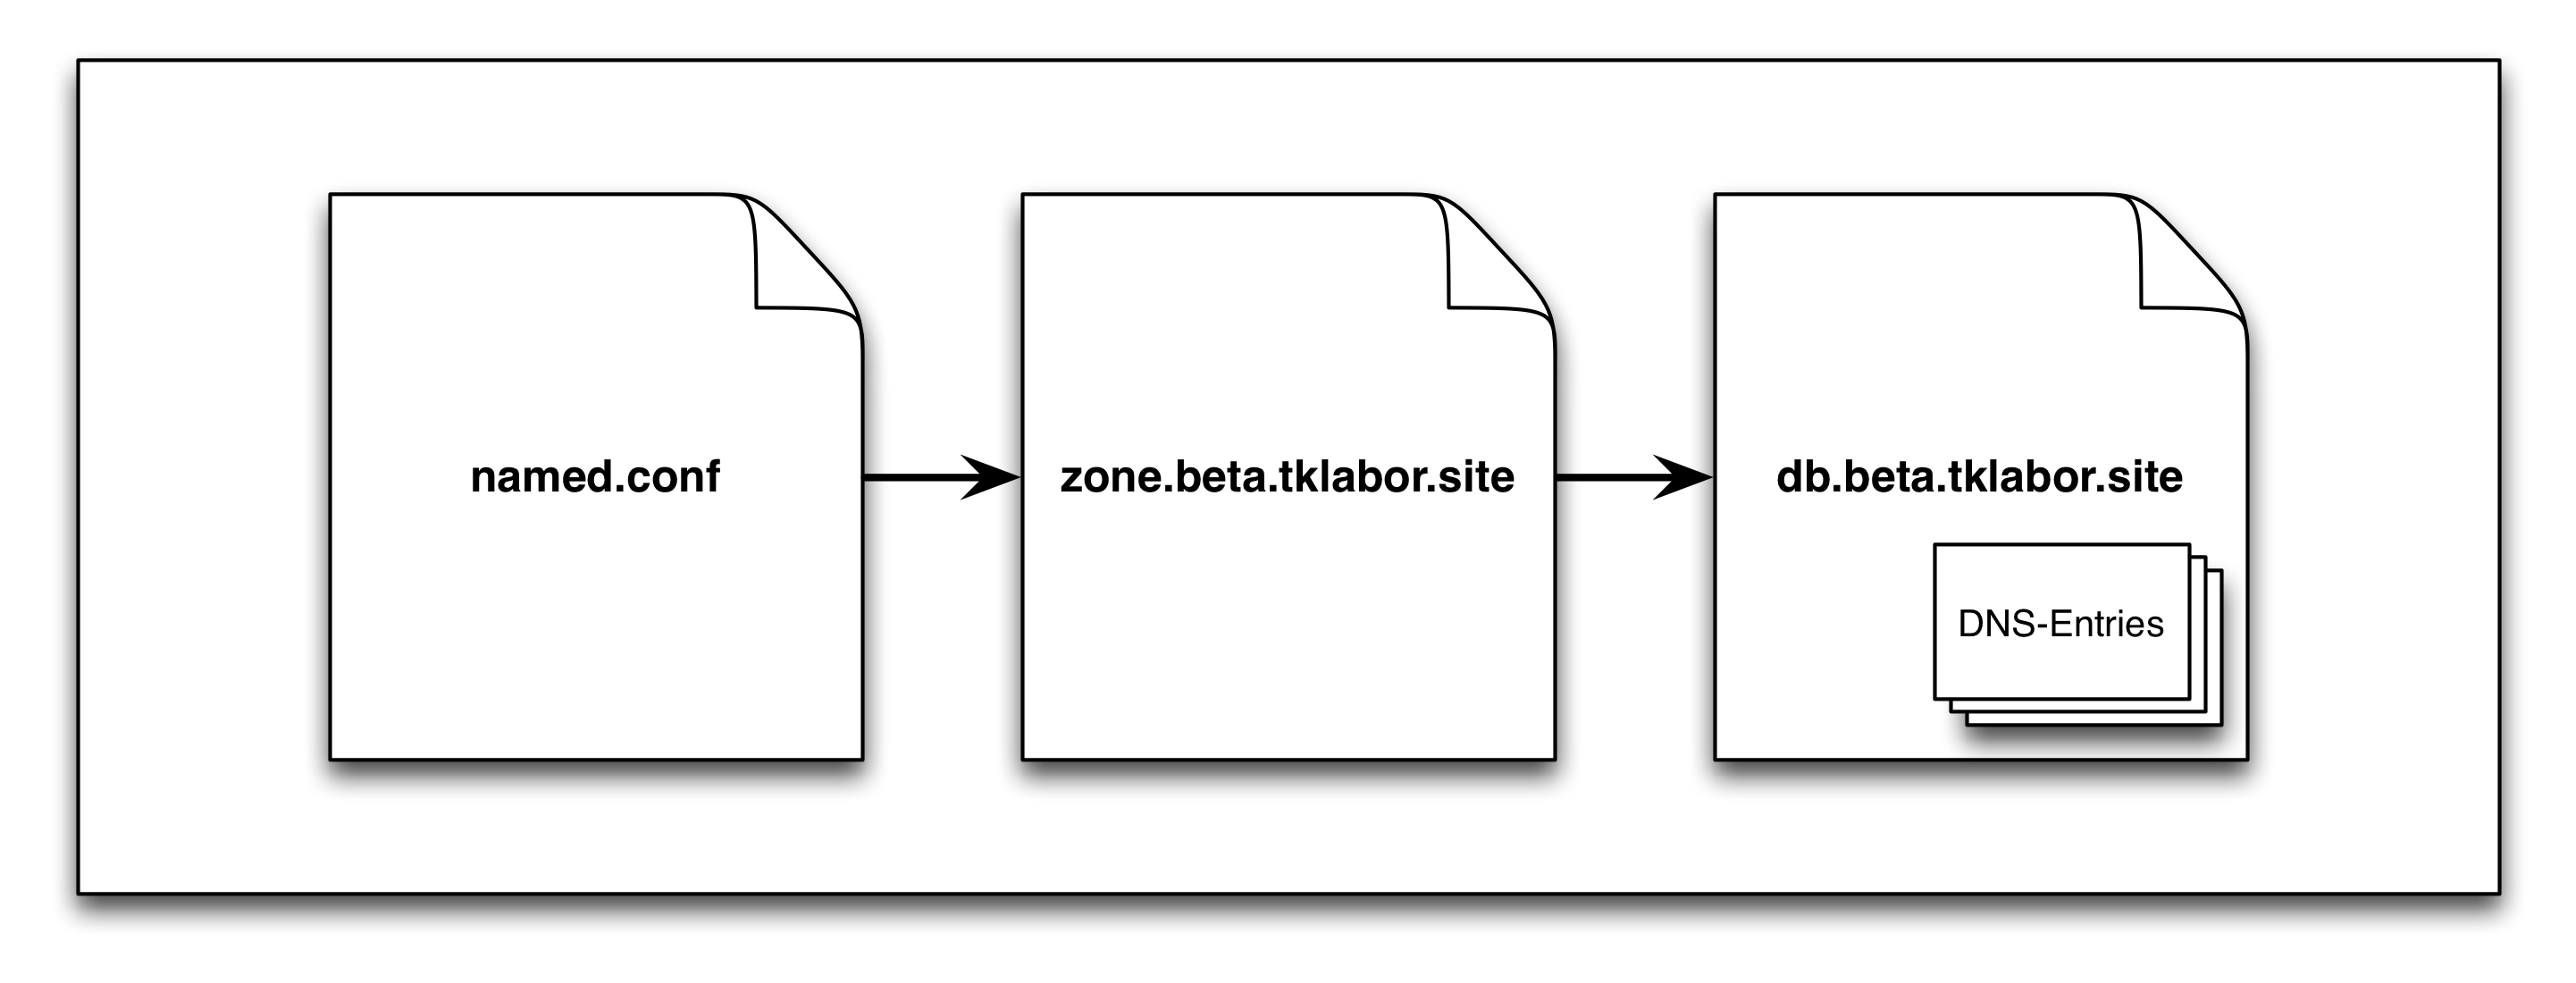
\includegraphics[width=0.85\textwidth]{images/dns-files.png}
	\end{center}
	\caption{Verweiskette der DNS-Zonenkonfiguration}
	\label{fig:bind-config-chain}
\end{nofloat}

Für die Zone \textbf{beta.tklabor.site} wird eine Zonendatei erstellt. Diese
Datei wird in der globalen Konfigurationsdatei von \textit{bind} wie folgt
inkludiert:

\begin{lstlisting}
admin1@srv200$ sudo vi /etc/bind/named.conf
\end{lstlisting}

Diese sollte dann folgendermaßen aussehen:

\begin{scriptsize}
\begin{lstlisting}
// This is the primary configuration file for the BIND DNS server named.
//
// Please read /usr/share/doc/bind9/README.Debian.gz for information on the 
// structure of BIND configuration files in Debian, *BEFORE* you customize 
// this configuration file.
//
// If you are just adding zones, please do that in /etc/bind/named.conf.local

include "/etc/bind/named.conf.options";
include "/etc/bind/named.conf.local";
include "/etc/bind/named.conf.default-zones";
include "/etc/bind/zone.beta.tklabor.site";
\end{lstlisting}
\end{scriptsize}

Für die Zone wird eine Datei \textbf{/etc/bind/zone.beta.tklabor.site} angelegt.

\begin{lstlisting}
admin1@srv200$ sudo vi /etc/bind/zone.beta.tklabor.site
\end{lstlisting}

\begin{scriptsize}
\begin{lstlisting}
zone "beta.tklabor.site" IN {
	type master;
	file "/etc/bind/db.beta.tklabor.site";
};
\end{lstlisting}
\end{scriptsize}

Im letzten Schritt muss eine Datenbank-Datei für die eigentlichen
Zonen-Einträge erstellt werden:

\begin{lstlisting}
admin1@srv200$ sudo vi /etc/bind/db.beta.tklabor.site
\end{lstlisting}

Diese sollte dann folgenden Inhalt haben:

\begin{scriptsize}
\begin{lstlisting}
$TTL 3600
$ORIGIN beta.tklabor.site.
;
; forward lookup for beta.tklabor.site
;
@    IN   SOA  ns.beta.tklabor.site. root.beta.tklabor.site. ( 
                 20110401 15m 5m 30d 1h
               )
     IN   NS   ns.beta.tklabor.site.

ns   IN   A    10.174.26.200
\end{lstlisting}
\end{scriptsize}

Jetzt stoppen und starten wir den entsprechenden Dienst:
\begin{lstlisting}
admin1@srv200$ sudo service bind9 restart
\end{lstlisting}

Um die Namensauflösung jetzt über den eigenen DNS-Server durchzuführen muss auf
beiden Servern der DNS-Server geändert werden. Die Abfragen werden nun nicht
mehr auf den 10.174.26.126 durchgeführt.
\begin{lstlisting}
admin1@srv200:~$ sudo vi /etc/resolv.conf
\end{lstlisting}

Die Datei sollte dann wie folgt aussehen:
\begin{scriptsize}
\begin{lstlisting}
nameserver 10.174.26.200
domain beta.tklabor.site
search beta.tklabor.site
\end{lstlisting}
\end{scriptsize}

In der Regel sollte es nun möglich sein den Nameserver der Domäne \textbf{beta.tklabor.site} zu ermitteln.

\begin{scriptsize}
\begin{lstlisting}
root@srv200:/etc/bind# dig ns beta.tklabor.site

; <<>> DiG 9.7.1-P2 <<>> ns beta.tklabor.site
;; global options: +cmd
;; Got answer:
;; ->>HEADER<<- opcode: QUERY, status: NOERROR, id: 40508
;; flags: qr aa rd ra; QUERY: 1, ANSWER: 1, AUTHORITY: 0, ADDITIONAL: 1

;; QUESTION SECTION:
;beta.tklabor.site.		IN	NS

;; ANSWER SECTION:
beta.tklabor.site.	3600	IN	NS	ns.beta.tklabor.site.

;; ADDITIONAL SECTION:
ns.beta.tklabor.site.	3600	IN	A	10.174.26.200

;; Query time: 0 msec
;; SERVER: 10.174.26.200#53(10.174.26.200)
;; WHEN: Wed Mar 30 18:17:40 2011
;; MSG SIZE  rcvd: 68
\end{lstlisting}
\end{scriptsize}

\subsection{Aufgabe}
\begin{enumerate}
  \item Beschreiben Sie den Inhalt der Datei \textbf{db.beta.tklabor.site}
  (SOA, TTL, NS, A, CNAME, PTR, TXT, AAAA)
  \item Welche Eintragstypen (Records) in einem Zonen-file möglich sind.
  \item Tragen Sie in die Zone \textbf{beta.tklabor.site} einen Alias
  für srv200 und srv201 ein.
  \item Erstellen Sie einen \textit{Canonical Name Record} für srv201 mit der
  Bezeichnung \textbf{www}.
  \item Konfigurieren Sie eine Reverse Lookup Zone für 10.174.26.0/24. Eine
  Zonendatenbankdatei als Beispiel finden Sie im Anhang auf Seite
  \pageref{cfg:bind-reverse-lookup}.
 \end{enumerate}

%------------------------------------------------------------------------------
\subsection{Funktionstest}
%------------------------------------------------------------------------------
Prüfen die folgenden Funktionen:
\begin{enumerate}
  \item Testen Sie die Namensauflösung für srv200.beta.tklabor.site und für
  srv201.beta.tklabor.site
  \item Testen Sie die Namensauflösung für www.beta.tklabor.site
  \item Testen Sie die Namensauflösung einer Internetdomain \textit{www.fsf.org}
  \item Testen Sie den Reverse Lookup für 10.174.26.200 mit \textit{nslookup}
  und \textit{dig}
  \item Testen Sie die oben genannte Namensauflösung mit \textit{dig +trace}.
  \item Wie verhält sich \textbf{dig @10.174.26.126 www.fsf.org} im Gegensatz zu
  \textbf{dig @10.174.26.200 www.fsf.org}?
\end{enumerate}
